\documentclass[journal,twocolumn]{IEEEtran}
\usepackage{graphicx,times,amsmath,amssymb,cite,subfigure,stfloats,booktabs, url,multirow,afterpage}
\usepackage[lined,ruled]{algorithm2e}
\usepackage{pifont}
\allowdisplaybreaks

\makeatletter
\newcommand{\rmnum}[1]{\romannumeral #1}
\newcommand{\Rmnum}[1]{\expandafter\@slowromancap\romannumeral #1@}
\makeatother


\begin{document}
\title{Exploring EEG Decoding with LLMs: A Purity-Guided Active Prompting Framework}

% \author{Dongrui~Wu,~\IEEEmembership{Fellow,~IEEE} and Jerry M. Mendel,~\IEEEmembership{Life Fellow, IEEE}
\author{Jingwei~Luo, Ziwei~Wang, Dingkun~Liu and Dongrui~Wu,~\IEEEmembership{Fellow,~IEEE}

\thanks{J.~Luo, Z.~Wang, D.~Liu, and D.~Wu, are with the Ministry of Education Key Laboratory of Image Processing and Intelligent Control, School of Artificial Intelligence and Automation, Huazhong University of Science and Technology, Wuhan, 430074 China.}
\thanks{D.~Liu and D.~Wu, are also with Zhongguancun Academy, Beijing, 100080 China.}
\thanks{J.~Luo, Z.~Wang, D.~Liu, and D.~Wu are also with the Shenzhen Huazhong University of Science and Technology Research Institute, Shenzhen, 518000 China.}
\thanks{Corresponding Authors: Dongrui Wu (drwu09@gmail.com).}
}
% \markboth{IEEE Transactions on Fuzzy Systems, 2023}%
\markboth{}%
{Shell \MakeLowercase{\textit{et al.}}: Bare Demo of IEEEtran.cls for IEEE Journals}
\maketitle

\begin{abstract}
Large language models (LLMs) have demonstrated impressive in-context learning (ICL) capabilities, particularly in few-shot prompting scenarios. However, most studies have concentrated on natural language processing (NLP) and computer vision (CV), with minimal exploration into domains involving complex physiologic signals such as electroencephalogram (EEG) decoding.
To bridge this gap, we propose a purity-guided active prompting (PGAP) framework, which integrates domain-specific EEG feature extraction with an active learning-based demonstration selection strategy. PGAP identifies a compact set of prototypical examples that effectively activate the few-shot capabilities of LLMs without requiring gradient-based parameter updates, and is compatible with both open-source and closed-source models.
Unlike the conventional framework that involves random demonstration selection on a per-instance basis for each test sample, PGAP performs a one-time identification of highly representative EEG samples from the training set, significantly reducing computational overhead.
Extensive experiments on seven EEG datasets and three paradigms demonstrate that PGAP consistently outperforms five existing sample selection baselines, achieving superior accuracy and robustness. Furthermore, performance improves with more powerful LLMs (e.g., DeepSeek-V3), and in some cases, even surpasses state-of-the-art supervised models.
\end{abstract}

\begin{IEEEkeywords}
Brain-computer interface, LLMs, active learning, prompt engineering, in-context learning
\end{IEEEkeywords}

\IEEEpeerreviewmaketitle

\section{Introduction}

Transformer-based large language models (LLMs) \cite{vaswani2017attention} have achieved remarkable progress across a wide range of natural language processing (NLP) tasks. As model scale increases, LLMs exhibit strong in-context learning (ICL) capabilities, enabling them to perform downstream tasks by conditioning on a few demonstration examples during inference, without any gradient-based parameter updates \cite{brown2020language}.

Brain-computer interfaces (BCIs) \cite{Lance2012, Wolpaw2002} enable direct communication between the human brain and external devices, allowing users to interact with environment through brain signals that reflect cognitive states or intentions \cite{he2019transfer}. Among BCI modalities, electroencephalography (EEG) is the most widely adopted due to its low cost, non-invasiveness, and ease of acquisition.

Despite ICL has been extensively studied in NLP and computer vision (CV), its application in BCI tasks, especially based on EEG signals, remains underexplored. To bridge this gap, it is essential to exploit strategies that effectively embed high-dimensional physiological signals into textual prompts suitable for LLM processing.

Prior efforts have investigated such integration in domains such as tabular data \cite{hegselmann2023tabllm, liu2025umman} and medical records \cite{liu2023large}, where numerical values often possess clear semantic meaning and can be easily verbalized. However, EEG signals lack such intrinsic semantic context. For instance, the value “16” in a clinical record may represent a patient’s age, while in EEG data it may simply denote a voltage amplitude at a specific time point, devoid of symbolic meaning.

The high temporal density and dimensionality of EEG signals further complicate the usage of LLMs. Directly feeding such dense and unstructured data into an LLM may lead to excessive token consumption, thereby limiting the model’s capacity to extract meaningful patterns. Moreover, EEG signals are inherently non-stationary, exhibit substantial cross-subject variability, and suffer from low signal-to-noise ratios, posing significant challenges for direct LLM-based analysis. An overview of LLM applications across various domains, with a particular emphasis on the challenges of EEG decoding, is shown in Fig.~\ref{fig:fig_intro}.

\begin{figure}[htbp]\centering
\subfigure[]{\label{fig:intro_cv} 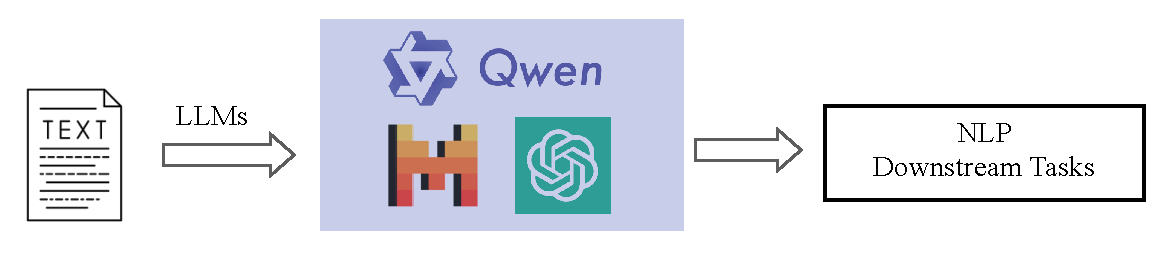
\includegraphics[width=\linewidth,clip]{intro_pic_nlp}}\\
\subfigure[]{\label{fig:intro_nlp} 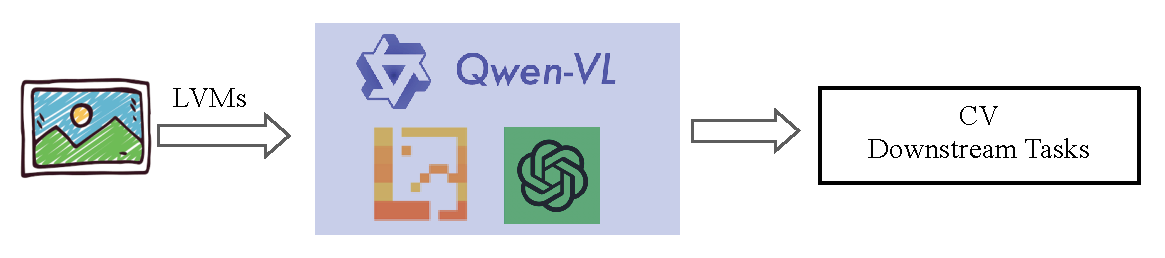
\includegraphics[width=\linewidth,clip]{intro_pic_cv}}\\
\subfigure[]{\label{fig:intro_eeg} 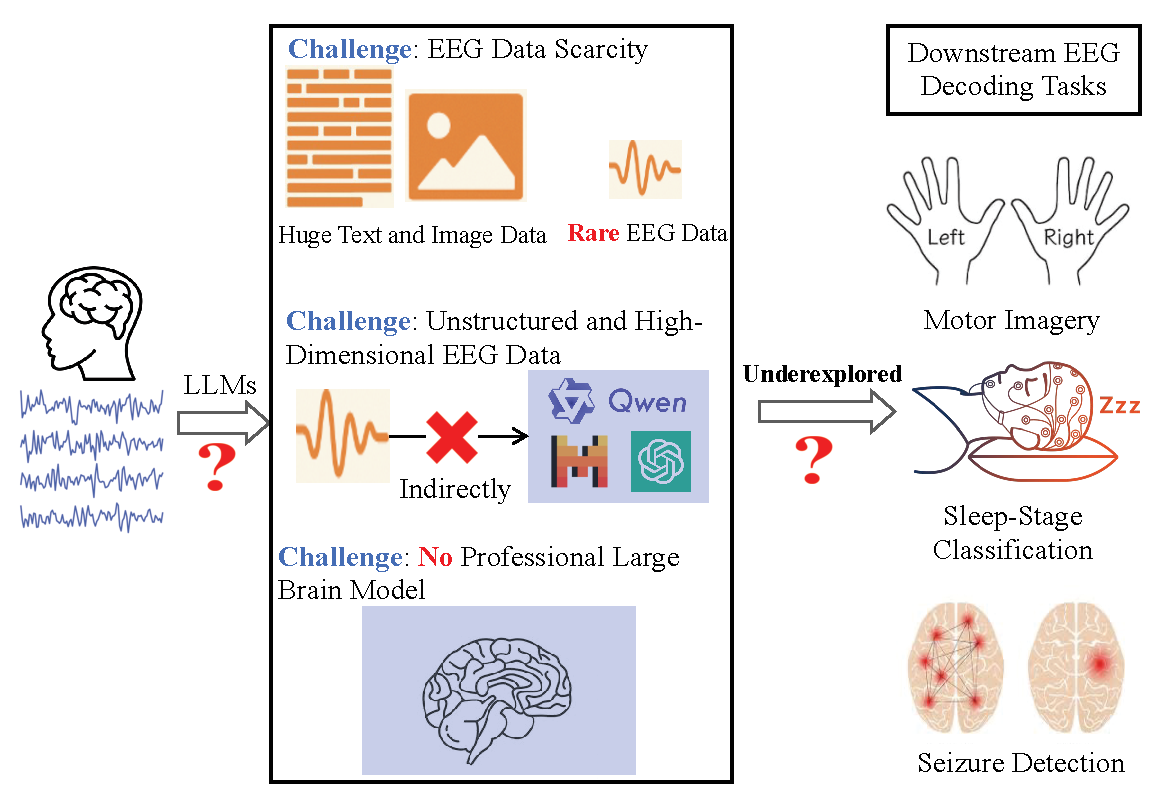
\includegraphics[width=\linewidth,clip]{intro_pic_eeg}}\\
\caption{LLM applications across various domains. (a) NLP; (b) CV; and (c) EEG decoding.} \label{fig:fig_intro}
\end{figure}

To address these challenges, we propose a simple yet effective purity-based active prompting (PGAP) framework that leverages domain-specific knowledge to extract compact and discriminative EEG representations suitable for LLM processing. Specifically, we introduce a purity-based example selection strategy that identifies highly consistent intra-class samples based on the $k$-nearest neighbor purity criterion. Experimental results on seven EEG datasets across three paradigms demonstrate that PGAP consistently outperforms existing sample selection algorithms.

In summary, our main contributions are as follows:
\begin{enumerate}
\item To the best of our knowledge, this work is the first attempt to harness LLMs for EEG signal classification through in-context few-shot prompting, thereby extending the applicability of LLMs to complex, low-semantic physiological domains beyond traditional text and vision tasks.
\item We incorporate neuroscience-informed feature extraction to reduce the input dimensionality and token count, enhancing both computational efficiency and downstream performance within the LLM-based prompting pipeline.
\item We propose a one-shot example selection strategy that identifies a fixed set of representative EEG samples from the training set and reuses them across all test instances, significantly reducing inference cost and latency compared to conventional per-instance prompting approaches.
\item Experiments on seven EEG datasets and three paradigms demonstrate that PGAP consistently outperforms existing sample selection approaches in both accuracy and robustness.
\end{enumerate}

The remainder of this paper is organized as follows: Section~\ref{sec:related} introduces related work. Section~\ref{sec:method} details the proposed PGAP. Section~\ref{sec:exp} presents the experimental results. Finally, Section~\ref{sec:conclusion} draws conclusions.


\section{Related Works}
\label{sec:related}

This section introduces related works of EEG decoding, active learning, and demonstration selection for ICL.
 
\subsection{EEG Decoding with Machine Learning}
EEG decoding encompasses a wide range of tasks, including motor imagery (MI) \cite{decety1996neurophysiological, liu2025spatial}, sleep stage classification \cite{aboalayon2016sleep}, and epilepsy detection \cite{wang2023tasa}. Traditional approaches typically rely on feature extraction approaches such as common spatial pattern (CSP) \cite{Ramoser2000}, frequency-domain features (e.g., power spectral density), time-domain features (e.g., amplitude statistics, zero-crossing rate), and entropy features (e.g., entropy, complexity measures) \cite{hassan2017automated}, followed by classifiers such as logistic regression (LR) \cite{cox1958regression}, support vector machines (SVM) \cite{cortes1995support}, etc.

To enhance EEG feature extraction, Ang \textit{et al.}~\cite{4634130} proposed the filter bank CSP (FBCSP) approach, which applies CSP to multiple frequency bands and automatically selects the most discriminative features for classification. Lotte \textit{et al.}~\cite{lotte2010regularizing} introduced regularized CSP to improve the robustness of feature extraction.

Recent advances in deep learning have enabled end-to-end models that jointly perform feature extraction and classification, achieving strong performance in EEG decoding tasks \cite{craik2019deep, shoeibi2021epileptic}. In particular, convolutional neural networks (CNNs) have demonstrated superior performance in MI classification. Schirrmeister \textit{et al.}~\cite{schirrmeister2017deep} proposed ShallowCNN, which uses temporal and spatial convolutional filters to extract discriminative representations for MI decoding. Lawhern \textit{et al.}~\cite{EEGNet} introduced EEGNet, a compact model employing depthwise and separable convolutions to significantly reduce the number of parameters while achieving strong performance across various BCI tasks, including MI classification. Song \textit{et al.} \cite{song2022conformer} proposed EEGConformer that sequentially integrates ShallowCNN with a Transformer block, facilitating high-level feature extraction. Wang \textit{et al.}~\cite{wang2025mvcnet} proposed MVCNet, a dual-branch network that parallelly integrates CNN and Transformer blocks to capture both local spatial-temporal features and global temporal dependencies, thereby enabling more informative feature extraction for MI decoding. Jiang \textit{et al.}~\cite{jiang2024csp} proposed CSP-Nets, a hybrid model that integrates knowledge-driven CSP filters with data-driven CNNs to improve MI classification performance.

More recently, Jiang \textit{et al.}~\cite{jiang2024large} proposed a 0.369B-parameter large-scale model trained on a diverse EEG corpus spanning multiple paradigms and tasks. However, due to the limited size of publicly available EEG datasets, model scalability remains constrained, and its performance and usability in downstream applications still fall short compared to LLMs. Additionally, due to the modality gap, no existing study has directly applied LLMs to EEG classification tasks via prompt-based ICL.

\subsection{Active Learning}

Traditional active learning (AL) algorithms primarily emphasized uncertainty-based sampling approaches, which prioritize samples near the decision boundary or those associated with high classification uncertainty \cite{Settles2009}. Lewis \textit{et al.}~\cite{lewis1995sequential} demonstrated that uncertainty sampling significantly reduces annotation costs in text classification tasks, outperforming both random and relevance sampling approaches, particularly when training data is limited.

Beyond uncertainty, representativeness has emerged as a complementary criterion. Strategies such as clustering-based sampling \cite{nguyen2004active} and density-weighted uncertainty sampling \cite{settles2008analysis} seek to select samples that are both uncertain and representative, avoiding outliers.

Multi-criteria approaches further enhance AL performance. Shen \textit{et al.}~\cite{Shen2004a} applied informativeness, representativeness, and diversity jointly to named entity recognition. Huang \textit{et al.}~\cite{huang2010active} introduced QUIRE, which selects samples by minimizing maximum model change (MMC), effectively balancing informativeness and representativeness. Cai \textit{et al.}~\cite{Cai2014} proposed a MMC strategy tailored to SVM, although it is sensitive to initial parameters. He \textit{et al.}~\cite{He2014} formulated a batch-mode AL approach combining uncertainty, representativeness, and diversity. Their approach quantifies informativeness as the product of uncertainty and representativeness, clusters samples via kernel k-means, and selects cluster centers for labeling.

In regression tasks, Burbidge \textit{et al.}~\cite{Burbidge2017} applied a query-by-committee (QBC) strategy based on model disagreement, though inaccurate model assumptions may degrade performance. Wu \textit{et al.}~\cite{wu2018pool}  proposed RD, a sequential pool-based approach that jointly considers representativeness and diversity. RD can be combined with existing regression-based AL approaches such as QBC, MCM, and Greedy sampling (GS) to further enhance performance. Wu \textit{et al.}~\cite{drwuiGS2019} further demonstrated that GS improves regression performance by maximizing sample diversity.

Despite its success in conventional machine learning, AL has been rarely applied to prompt selection in LLMs. Whether the selection criteria developed for conventional models remain effective in few-shot prompting scenarios with LLMs remains an open question.

\subsection{Demonstration Selection for ICL}
ICL, a paradigm wherein models learn tasks from a few example demonstrations without parameter updates \cite{dong-etal-2024-survey, achiam2023gpt}. With the scaling of model and data sizes, LLMs have demonstrated the ability to perform ICL. Most existing approaches to demonstration selection adopt a per-instance strategy, where demonstrations are selected independently for each test instance. This leads to two key selection objectives: similarity and diversity \cite{luo2024context}.

Liu \textit{et al.}~\cite{liu-etal-2022-makes} proposed selecting demonstrations based on similarity by retrieving the $k$ nearest neighbors of the test instance using sentence encoders in the embedding space. However, this approach does not consider diversity, which may result in homogeneous and redundant examples. Moreover, in classification tasks, $k$NN-based selection often biases the model toward predicting the majority label among the selected examples, effectively reducing the LLM to a $k$NN classifier and diminishing its unique generalization capabilities.

To address the issue of homogeneity, Li \textit{et al.}~\cite{li-etal-2024-self-prompting} introduced clustering-based retrieval, where the sample pool is first clustered, and the nearest instance to the query is selected from each cluster. While this approach increases diversity, it may include examples that lack sufficient similarity to the query.

To better balance similarity and diversity, iterative retrieval approaches have been proposed. These approaches begin by selecting the example most similar to the query and then sequentially add examples by considering both their similarity to the query and their diversity relative to previously selected samples. Scarlatos \textit{et al.}~\cite{scarlatos2023reticl} trained an long short-term memory (LSTM) based retriever within a reinforcement learning framework. During inference, the retriever selects an initial demonstration by processing the query, then updates the query representation using the LSTM's hidden state to incorporate prior demonstrations. This iterative process continues until $k$ demonstrations are selected \cite{luo2024context}. In CV, similar principles have been applied by scoring candidates using similarity metrics (e.g., cosine distance) to quantify relevance for prompt inclusion \cite{zhang2023makes}. In contrast to per-instance approaches, Hong \textit{et al.}~\cite{hongjin2022selective} proposed a two-step approach: first, a diverse and representative subset is selected for annotation; then, task-specific demonstrations are retrieved from this labeled pool at inference.

Overall, existing work on ICL demonstration selection has primarily focused on NLP and CV tasks, with strategies largely centered on balancing similarity and diversity among examples. Designing principled selection criteria for complex, non-semantic inputs, like EEG, presents a significant challenge.

\section{Method}\label{sec:method}

This section introduces the proposed PGAP. Specifically, we start with a large pool of labeled training samples and select a compact subset to serve as in-context examples within the prompt, aiming to fully leverage the few-shot capabilities of the LLM and maximize its performance on the test set. The overall procedure is illustrated in Figure~\ref{fig:flowchart}.

\begin{figure*}[htbp]
  \centering
  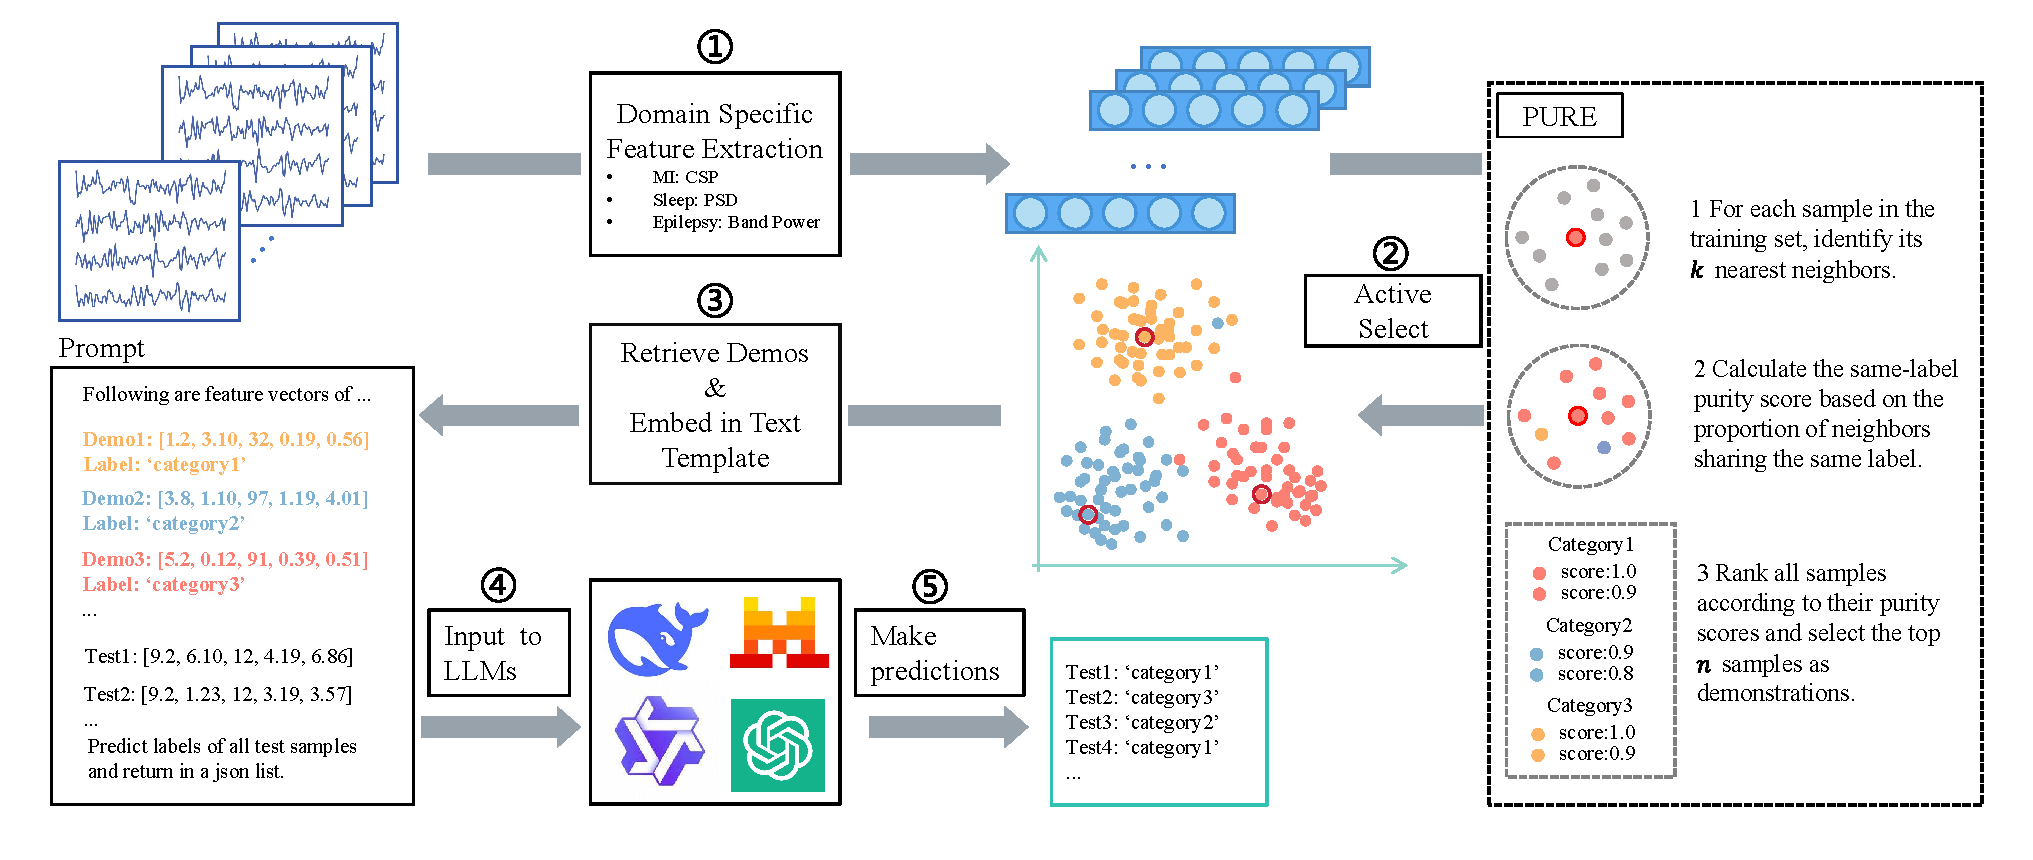
\includegraphics[width=1.0\linewidth, clip]{Fig1.eps}
  \caption{Flowchart of EEG-based classification using LLM few-shot prompting.}
  \label{fig:flowchart}
\end{figure*}

\subsection{Domain Specific Feature Extraction}

Due to the inherent complexity of raw EEG signals, it is essential to extract compact and discriminative handcrafted features following standard preprocessing. This step is crucial not only for enhancing task-relevant signal characteristics but also for reducing input dimensionality to meet the token-length constraints of LLMs. The resulting embeddings are subsequently utilized as demonstrations within the in-context prompt.

Domain-specific knowledge needs to be leveraged to design feature extraction pipelines tailored to different EEG paradigms. MI paradigm primarily elicits event-related desynchronization and synchronization patterns in the $\mu$ (8--13~Hz) and $\beta$ (13--30~Hz) frequency bands over the sensorimotor cortex, particularly around electrodes C3 and C4. We adopt a feature extraction pipeline inspired by the FBCSP framework~\cite{4634130} for MI EEG decoding. Specifically, signals are bandpass-filtered in the 8--24~Hz range and divided into four 4-Hz sub-bands:
\begin{align}
    \mathcal{B}_1 &= [8, 12]\,\text{Hz}, \notag \\
    \mathcal{B}_2 &= [12, 16]\,\text{Hz}, \notag \\
    \mathcal{B}_3 &= [16, 20]\,\text{Hz}, \notag \\
    \mathcal{B}_4 &= [20, 24]\,\text{Hz}. \notag
\end{align}

Given a multi-channel EEG trial $\mathbf{X}_{i} \in \mathbb{R}^{C \times T}$, where $i$ is the class index, $C$ the number of channels, and $T$ the number of time points, each sub-band signal $\mathbf{X}_{i}^{k}$ is obtained via bandpass filtering:
\begin{equation}
    \mathbf{X}_{i}^{k} = \mathrm{BandpassFilter}(\mathbf{X}_{i}, \mathcal{B}_k), \quad k=1,2,3,4.
    \label{eq:bandpass}
\end{equation}

Fig~\ref{fig:filterband} illustrates the filtered bands from an EEG trial at channel C3.
\begin{figure}[htbp]
  \centering
  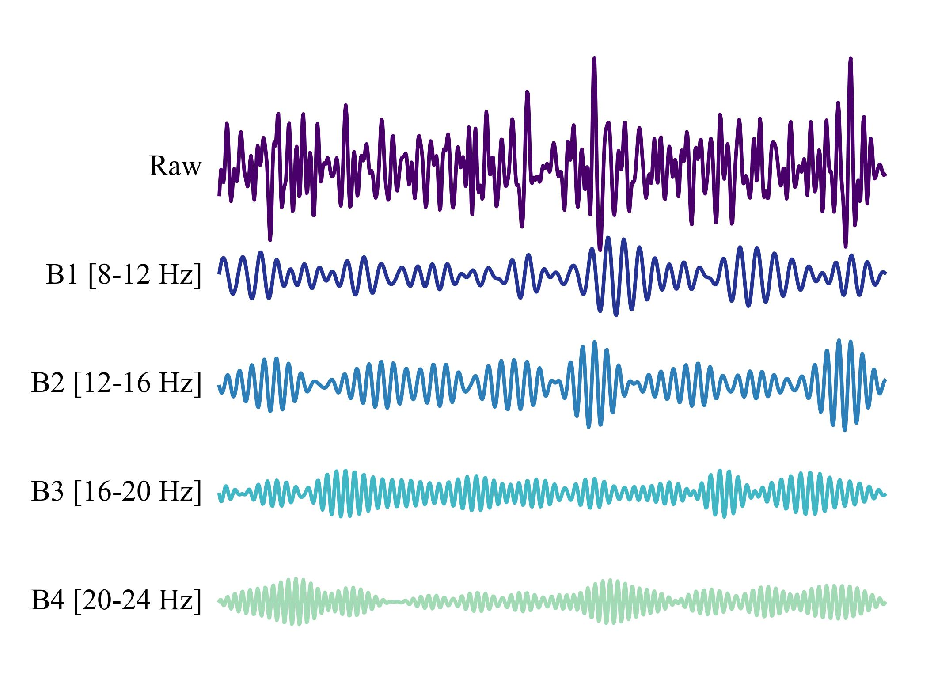
\includegraphics[width=1.0\linewidth, clip]{Fig4.eps}
  \caption{EEG signal from channel C3 and its band-specific components.}
  \label{fig:filterband}
\end{figure}

The CSP algorithm computes a spatial filtering matrix $W \in \mathbb{R}^{C \times C'}$ ($C' < C$) that reduces the dimensionality of EEG trials and improves class separability.

The mean spatial covariance matrix for class $i$ is calculated as:
\begin{equation}
    \Sigma_i = \frac{1}{N_i} \sum_{j=1}^{N_i} \frac{\mathbf{X}_{i,j}\mathbf{X}_{i,j}^\top}{\mathrm{tr}(\mathbf{X}_{i,j}\mathbf{X}_{i,j}^\top)},
    \label{eq:cov}
\end{equation}
where $\mathbf{X}_{i,j}$ denotes the $j$-th EEG trial of class $i$ and $N_i$ is the total number of trials in class $i$.

The spatial filter matrix $W$ is derived by maximizing (or minimizing) the following objective function:
\begin{equation}
    J(W) = \frac{W^\top \Sigma_1 W}{W^\top \Sigma_2 W},
    \label{eq:csp_obj}
\end{equation}
where $\Sigma_1$ and $\Sigma_2$ are the mean spatial covariance matrices of all EEG trials from two classes in MI, respectively.

The CSP features for a given band-filtered trial $\mathbf{X}^{k}$ are then computed by projecting the trial with the spatial filter $W$:
\begin{equation}
    \mathbf{Z}^{k} = W^\top \mathbf{X}^{k}
    \label{eq:csp_proj}
\end{equation}
and extracting the log-variance of each projected component:
\begin{equation}
    \mathbf{f}^{k} = \log \left( \frac{\mathrm{var}(\mathbf{Z}^{k}_r)}{\sum_{l=1}^{C'} \mathrm{var}(\mathbf{Z}^{k}_l)} \right), \quad r=1,\ldots,C',
    \label{eq:csp_feat}
\end{equation}
where $\mathrm{var}(\cdot)$ denotes the temporal variance of the $r$-th spatially filtered signal.

Finally, all CSP features from the four sub-bands are concatenated to form an 8-dimensional feature vector for each trial:
\begin{equation}
    \mathbf{f} = [\mathbf{f}^{1},\ \mathbf{f}^{2},\ \mathbf{f}^{3},\ \mathbf{f}^{4}].
    \label{eq:concat_feat}
\end{equation}

For sleep stage classification, EEG features can be extracted from the time, frequency, and time-frequency domains. In the time domain, standard statistical features such as amplitude measures and zero-crossing rates are commonly employed. In the frequency domain, power spectral density (PSD) and band power features are widely used. Time-frequency features are often obtained using approaches such as wavelet transform, short-time Fourier transform, empirical mode decomposition, and Wigner–Ville distribution. Given that our primary goal is to evaluate the impact of demonstration selection strategies (random vs. active), we focus on the delta (0.5--4~Hz), theta (4–8~Hz), alpha (8--13~Hz), spindle (12--14~Hz), and beta (14--30~Hz) bands, which have been shown in the literature to correspond to sleep stages W, N1--N3, and REM.

We adopt a simple yet effective feature representation based on multi-band PSD analysis. Given a multi-channel EEG trial $\mathbf{X} \in \mathbb{R}^{C \times T}$, the signal is first decomposed into a set of standard frequency bands $\{\mathcal{B}_k\}$, where each $\mathcal{B}_k$ corresponds to a specific frequency range of interest. For each channel $c$ and frequency band $k$, the PSD feature is obtained by estimating the spectral distribution $S_c(f)$ (e.g., via Welch's method), and subsequently averaging the spectral power within the target frequency range: 
\begin{equation}
    \mathrm{PSD}_{c,k} = \frac{1}{N_k} \sum_{f_j \in \mathcal{B}_k} S_c(f_j),
    \label{eq:psd_feature}
\end{equation}
where $S_c(f_j)$ is the estimated PSD value at frequency $f_j$, and $N_k$ the number of frequency bins within the band $\mathcal{B}_k$. The feature vector for each trial is then formed by concatenating the PSD features across all channels and selected frequency bands:
\begin{equation}
    \mathbf{f} = [\mathrm{PSD}_{1,1}, \ldots, \mathrm{PSD}_{1,K}, \mathrm{PSD}_{2,1}, \ldots, \mathrm{PSD}_{C,K}],
    \label{eq:feature_vector}
\end{equation}
where $K$ is the number of bands and $C$ is the number of channels.

For epileptic seizure detection, previous studies have explored various domain features~\cite{wang2023tasa,boonyakitanont2020review}, highlighting the effectiveness of amplitude-based representations such as variance, energy, and entropy. Motivated by these insights, we adopt a practical and compact feature representation by computing band-specific signal power directly from raw EEG signals. Specifically, we apply bandpass filters to decompose the signals into canonical frequency bands: $\delta$ (0.5--4~Hz), $\theta$ (4--8~Hz), $\alpha$ (8--13~Hz), $\beta$ (13--30~Hz), and $\gamma$ (30--45~Hz). Then, the average power is extracted from each band. This approach effectively captures band-level spectral energy patterns, which are highly indicative of seizure-related dynamics, while maintaining low computational complexity.

Mathematically, for each frequency band $\mathcal{B}_k$, we obtain the band-filtered signal:
\begin{equation}
    \mathbf{X}^{(k)} = \mathrm{BandpassFilter}(\mathbf{X}, \mathcal{B}_k),
    \label{eq:band_filter}
\end{equation}
where $\mathcal{B}_k$ denotes the $k$-th frequency band. The instantaneous power for channel $c$ in band $k$ is computed as:
\begin{equation}
    P_{c,k}(t) = \left[\mathbf{X}^{k}_{c, t}\right]^2,
    \label{eq:inst_power}
\end{equation}
and the average power over time for each channel and band is:
\begin{equation}
    \overline{P}_{c,k} = \frac{1}{T} \sum_{t=1}^{T} P_{c,k}(t) = \frac{1}{T} \sum_{t=1}^{T} \left[\mathbf{X}^{k}_{c, t}\right]^2.
    \label{eq:avg_band_power}
\end{equation}
To obtain a compact representation, the mean power across all channels is further computed for each band:
\begin{equation}
    \overline{P}_{k} = \frac{1}{C} \sum_{c=1}^{C} \overline{P}_{c,k}.
    \label{eq:pool_band_power}
\end{equation}
Finally, the feature vector for each trial is constructed as:
\begin{equation}
    \mathbf{f} = [\overline{P}_{1}, \overline{P}_{2}, \ldots, \overline{P}_{B}],
    \label{eq:feature_vector_band_power}
\end{equation}
where $B$ is the number of frequency bands.


\subsection{PGAP}
\label{subsec:PGAP}

After obtaining compact feature vectors, we proceed to select a small subset of examples that most effectively activate the few-shot learning capabilities of the LLM. However, as previously mentioned, it remains unclear whether principles from conventional AL are directly applicable to EEG-based decoding with LLMs. To address this, we conducted a series of experiments to systematically evaluate the effectiveness of different example selection strategies.

Contrary to prevailing assumptions, our findings reveal that the most informative samples, such as those located near the decision boundary or associated with high prediction uncertainty, did not yield optimal performance. Instead, the most confidently predicted samples, which are typically less informative in traditional active learning, consistently led to superior decoding performance. This observation supports our hypothesis that high-uncertainty examples may introduce ambiguity and provide suboptimal guidance during inference. In contrast, prototypical and easily classifiable examples more faithfully capture the intrinsic characteristics of their respective classes, thereby supporting more accurate model predictions.

Motivated by this insight, we propose PGAP, a simple yet effective pipeline for selecting in-context examples in EEG-based tasks. For each training sample, we compute its $k$ nearest neighbors and calculate the proportion of neighbors that share the same class label, a metric we refer to as local same-label purity. As illustrated in Algorithm~\ref{alg:PGAP}, all training samples are ranked by their purity scores, and the top-$n$ most “PGAP” samples are selected as in-context examples. This selection strategy favors the most representative samples within each class while inherently filtering out outliers, which tend to be surrounded by mixed-class neighbors and thus receive lower purity scores.

Although PGAP does not explicitly enforce diversity, we empirically observe that augmenting it with greedy diversity sampling leads to performance degradation. This indicates that, in the context of LLM-based EEG decoding, purity alone serves as a more effective selection criterion for example selection.

PGAP adopts a one-time selection strategy, in which a fixed set of in-context examples is selected once from the training set and reused across all test instances. Compared to conventional per-instance selection, this approach offers significant computational benefits:

\begin{enumerate}
  \item \emph{Reducing computational overhead:} PGAP eliminates the need for dynamic retrieval by avoiding repeated exemplar selection for each test instance.
  \item \emph{Improving batch efficiency:} Since all test samples share the same in-context examples, multiple test inputs can be batched into a single prompt, enabling parallel predictions with a single API call. In contrast, per-instance selection requires individualized prompt construction, allowing only one prediction per query.
\end{enumerate}

\subsection{Prompt Design}

The final step involves constructing the in-context prompt by combining the selected examples and their corresponding labels together with the task description, contextual information, and explicit output instructions. This prompt is then presented to the LLM alongside the test input.

Our design follows established best practices in prompt engineering to ensure clear and effective communication with the LLM \cite{chen2023unleashing}. Specifically, the task description is concise, unambiguous, and positioned at the beginning of the prompt to explicitly define the model's objective. The context section incorporates relevant background information and a few representative input–output pairs, enabling the model to infer the underlying mapping pattern from demonstrations.

To further guide the model toward producing consistent and structured outputs, explicit output instructions are incorporated. These instructions specify both content constraints (e.g., label formats, output options) and style constraints (e.g., use of quotation marks, line breaks), which are critical for downstream evaluation and integration. Additionally, we employ prompt formatting techniques such as section delimiters (e.g., “\#\#\#” or newline markers), standardized indentation, and token normalization to delineate boundaries between different components, including descriptions, examples, and the query, thereby improving prompt clarity and model interpretability. A typical prompt structure used in our study is shown in Fig~\ref{fig:template}.

To avoid prompt truncation and exceeding token limits, all components are carefully optimized for brevity while preserving essential information. This balance is particularly critical when interacting with token-limited APIs or processing long test inputs. The final prompt format is compatible with both open-source and API-based LLMs and is designed to support reusable, batch-level inputs for efficient inference.

\begin{algorithm}[ht]
  \caption{PGAP}
  \label{alg:PGAP}
  \KwIn{
      N labeled samples, $\{\mathbf{x}_n\}_{n=1}^N$, where $\mathbf{x}_n \in \mathbf{R}^d$;\\
      \hspace*{3.1em} $C$, number of classes; \\
      \hspace*{3.1em} $M$, number of samples to select; \\
      \hspace*{3.1em} $K$, neighborhood size
  }
  \KwOut{A list of selected sample indices with balanced class distribution $L$.}
  
  Ensure $M$ is divisible by $C$; \\

  \ForEach{sample $n = 1$ to $N$}{
      Compute distances between $\mathbf{x}_n$ and all other samples; \\
      Find $K$ nearest neighbors of $\mathbf{x}_n$ (excluding itself); \\
      Compute same-label purity score:
      \[
      \text{purity}(\mathbf{x}_n) = \frac{\text{Number of same-label neighbors}}{K}
      \]
  }
  Group all samples by class label; \\
  Sort each group in descending order of purity score; \\
  \ForEach{class $c = 1$ to $C$}{
      Select top $M / C$ samples with highest purity; \\
      Add their indices to output list $L$;
  }
  \Return{Selected sample indices list $L$.}
\end{algorithm}

\begin{figure}[htbp]
  \centering
  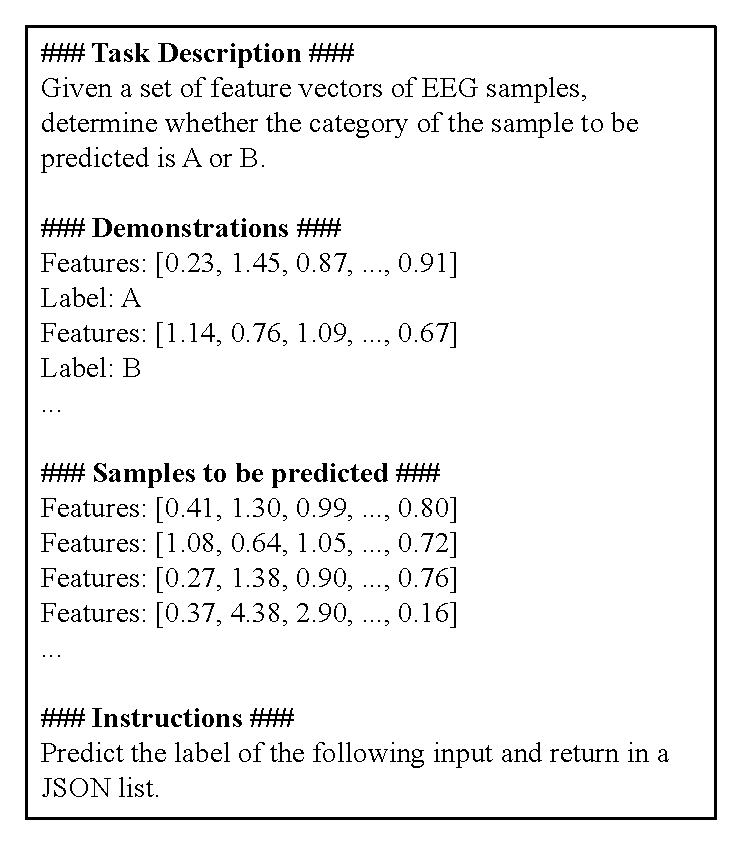
\includegraphics[width=1.0\linewidth, clip]{Fig2.eps}
  \caption{A typical prompt structure used in our experiments.}
  \label{fig:template} 
\end{figure}


\begin{table*}[htpb] \centering
  \caption{Summary of the seven EEG datasets.}
  \label{tab:datasets}
  \begin{tabular}{c|c|c|c|c|c|c|c}
  \toprule
  BCI&\multirow{2}{*}{Dataset} & Number of & Number of & Sampling & Trial Length & Number of Trials  & \multirow{2}{*}{Class Labels} \\
  Paradigm& & Subjects & Channels & Rate (Hz) & (seconds) & per Subject &  \\
  \midrule
  \multirow{4}{*}{MI}&BNCI2014001 & 9 & 22 & 250 & 4  & 288 &  left hand, right hand \\
  &BNCI2014004 & 9 & 3 & 250 & 4.5 & 680-760 &  left hand, right hand \\
  &BNCI2014002 & 14 & 15 & 512 & 5 & 160 &  right hand, both feet \\
  &BNCI2015001 & 12(9) & 13 & 512 & 5 & 400/600 &  right hand, both feet \\
  &Weibo2014 & 10 & 60(22) & 200 & 4 & 140, 160 &  right hand, both feet \\
  \midrule
  Sleep&Sleep-EdfX& 7 & 2 & 100 & 30 & 1025 &  W, N1, N2, N3, REM \\
  \midrule
  Epilepsy&CHB-MIT&10&23&256&3&76-618&seizure, non-seizure \\
  \bottomrule
  \end{tabular}
\end{table*}


\section{Experiments and Results}\label{sec:exp}
\subsection{Datasets}
Five MI datasets, one sleep dataset, and one epilepsy dataset are utilized in our experiments.

\subsubsection{MI Datasets}
All MI datasets used in our experiments are binary classification tasks and were obtained using the MOABB framework \cite{jayaram2018moabb}. Specifically, two datasets from BCI Competition IV (BNCI2014001 and BNCI2014004) \cite{tangermann2012review} contain left-vs-right hand imagery, while the other three: BNCI2014002, BNCI2015001, and Weibo2014, contain right-hand vs. feet imagery. 

In each session, a subject sat comfortably in an armchair positioned in front of a computer screen. At the beginning of each trial, a fixation cross appeared on a black background, accompanied by a short auditory warning tone. After a brief delay, a directional cue in the form of an arrow pointing left, right, down, or up appeared on the screen, corresponding to one of the four MI classes: left hand, right hand, feet, or tongue. Subjects performed the imagery task until the fixation cross disappeared. Each trial ended with a brief black screen before the next trial began \cite{tangermann2012review}.

Notably, for BNCI2015001, the last 3 subjects were excluded due to poor performance \cite{faller2012autocalibration}. And for Weibo2014, only right-hand and feet trials were used for binary classification in this study. From the original 60 usable channels, we selected 21 MI-related channels: FC3, FC1, FCz, FC2, FC4, C5, C3, C1, Cz, C2, C4, C6, CP3, CP1, CPz, CP2, CP4, P3, P1, P2, and P4.


\subsubsection{Sleep Dataset}
The Sleep-EDF Expanded (Sleep-EDFx) dataset is intended for sleep research, particularly for sleep stage classification. It contains 197 full-night polysomnographic (PSG) recordings, including EEG (Fpz–Cz and Pz–Oz), EOG, EMG, and event markers. Corresponding hypnograms (sleep stage annotations) were manually scored by trained technicians following the Rechtschaffen and Kales manual and are provided alongside the recordings.

Only EEG channels are used for a five-stage sleep classification task. Due to the large volume of data, we selected recordings from the first seven subjects, using one night of data per subject.

During the signal processing and feature extraction stages, EEG data from the Sleep-EDFx dataset were first bandpass filtered between 0.5 Hz and 35 Hz. Since the recordings span an entire night and include prolonged wake periods at the beginning and end, only the first and last 30 minutes of wakefulness were retained to reduce redundancy. Sleep stages were labeled according to the AASM standard and grouped into five classes: Wake (W), N1, N2, N3, and REM. Each trial was segmented into non-overlapping 30-second epochs.

For each epoch, the signal from every channel was processed individually. The PSD was computed using the Welch algorithm. We then defined five canonical frequency bands-delta (0.5-4 Hz), theta (4-8 Hz), alpha (8-13 Hz), spindle (12-14 Hz) and beta (14-30 Hz). For each band, the mean PSD within the corresponding frequency range was calculated by averaging the PSD values across that band. This process was repeated across all channels and frequency bands, resulting in a feature vector of size $C \times B$ per epoch, where $C$ is the number of EEG channels and B is the number of frequency bands.

\subsubsection{Epilepsy Dataset}
The CHB-MIT Scalp EEG Database comprises EEG recordings from 22 pediatric subjects (5 males, aged 3–22 years, and 17 females, aged 1.5-19 years) with intractable seizures. Subjects were monitored over multiple days following the withdrawal of anti-seizure medication to capture seizure activity and evaluate their suitability for surgical intervention. In total, 182 seizures were annotated with precise onset and offset timings.

All signals were sampled at 256 Hz with 16-bit resolution. Most recordings contain 23 EEG channels, though a few have 24 or 26. Electrode placement follows the International 10-20 system for EEG acquisition.

Considering the computational cost, we only used the first ten subjects in our experiments. The raw EEG signals were segmented using non-overlapping sliding windows of 3 seconds. We extracted all seizure segments and randomly selected an equal number of non-seizure segments from the remaining data. During inference, the number of seizure and non-seizure trials was also equal, thus avoiding class imbalance.

For feature extraction, we employed a commonly used and effective time-domain features for seizure detection: band power. Specifically, the raw EEG signals were filtered into five standard frequency bands: $\delta$ (0.5–4 Hz), $\theta$ (4–8 Hz), $\alpha$ (8–13 Hz), $\beta$ (13–30 Hz), and $\gamma$ (30–50 Hz). 

For each frequency band, the signal from every channel was individually filtered and the power was calculated as the mean squared amplitude over time. The power values from all channels were then averaged to obtain a single scalar representing the overall energy in that frequency band. This process was repeated for all five bands, resulting in a five-dimensional feature vector per EEG epoch. These band power features provide a compact summary of the frequency-specific signal energy across the scalp.

\subsection{Compared Approaches}
We compare PGAP with various existing approaches:
\begin{enumerate}
\item \emph{BL}, which randomly selects all $M$ samples.
\item \emph{CTD}, which applies the $k$-means algorithm within each class and selects centroids.
\item \emph{RD} \cite{wu2018pool}, which starts by selecting the centroid of each class as the initial point. Then, iteratively performs additional rounds of clustering on each class and selects the centroid of the largest cluster not yet covered by the previously selected points.
\item \emph{SVM-near}, which trains an SVM classifier on the training set and selects, from each class, the sample closest to the decision boundary.
\item \emph{SVM-far}, in contrast to SVM-near, selects the sample farthest to the decision boundary within each class. To mitigate the impact of outliers, SVM-far further filters candidates by checking the proportion of same-label samples among their five nearest neighbors.
\item \emph{PGAP}, which selects the highest-purity samples from each class, as described in Section~\ref{subsec:PGAP}.
\end{enumerate}

\subsection{Implementation}
We utilize the Qwen-2.5-14B-Instruct-1M model as the LLM, and apply two demonstrations per category, resulting in a total of four ICL demonstrations for the MI binary classification dataset, ten for the sleep five-class classification task, and four for the epilepsy binary classification dataset.

We conducted experiments under three settings. For the MI datasets, we adopted within-subject cross-session and cross-subject evaluation. For sleep and epilepsy datasets, as only one session per subject is available, we employed within-subject five-fold cross-validation instead of cross-session evaluation. For the epilepsy dataset, due to the large variation in the number of seizure segments across subjects, we only conduct within-subject experiments.

All algorithms were run 5 times, except random selection, which was repeated 20 times. For five-fold cross-validation, the entire process was repeated 5 times, totally 25 runs for each approach. Classification accuracy was utilized as the evaluation metric.

\begin{enumerate}
\item \emph{Within-subject cross-session:}
Datasets were partitioned into non-overlapping training and testing sets. Specifically:
  \begin{itemize}
	\item BNCI2014001: One session for training and another for testing, each containing 144 trials.
	\item BNCI2014004: First 3 sessions for training; last 2 for testing.
    \item BNCI2014002: First 5 runs for training; last 3 for testing. Each run contains 10 right-hand and 10 feet trials.
    \item BNCI2015001: One session for training and one for testing (400 trials total). Subjects 8–9 use first 2 sessions for training and the third for testing.
    \item Weibo2014: First half of the session for training; second half for testing.
  \end{itemize}
  \item \emph{Within-subject five-fold cross-validation:}
Trials from each subject were shuffled and split into 5 folds with class balance preserved.
  \item \emph{Leave one subject out:} Remaining subjects used for training. Euclidean Alignment (EA) \cite{he2019transfer} was applied to each subject's data.
\end{enumerate}

\subsection{Main Results}
Tables~\ref{tab:2014001-result}-\ref{tab:chb-mit-result} presents the classification accuracies on the seven EEG datasets, respectively. Observe that:
\begin{enumerate}
  \item {Active selection of ICL demonstrations significantly outperforms random selection.} In both within-subject and cross-subject settings, actively selected demonstrations consistently lead to a better prompting effect on the LLM, resulting in higher prediction accuracy and more stable outputs compared to random selection.
  \item {High-informativeness samples yield the worst prompting effect in ICL.} Contrary to conventional expectations in traditional machine learning, selecting the most informative samples leads to an inferior prompting effect on the LLM, even worse than random selection. This suggests a fundamental difference between how LLMs and traditional classifiers benefit from informative instances.
  \item {Low-informativeness samples achieve the best prompting effect.} Demonstrations with low informativeness and high model confidence, as exemplified by SVM-far and PGAP, result in superior prompting effects. We hypothesize that when classifying complex numerical data, LLMs primarily rely on statistical distributional patterns rather than constructing deep decision boundaries. Therefore, more prototypical and easily distinguishable examples are more effective in guiding the model, whereas highly ambiguous samples fail to provide meaningful distinctions.
  \item {PGAP consistently outperforms SVM-far.} Although SVM-far has been optimized to avoid outlier selection and shows competitive performance, PGAP still achieves better overall prompting effects across datasets and experimental conditions.
  \item {PGAP achieves consistent superiority across multiple datasets and paradigms.} The proposed PGAP consistently outperforms random selection across all experiments and achieves optimal results in the majority of cases. Specifically, in the within-subject setting, PGAP improves over random selection by 8.04\%, 8.19\%, 6.03\%, 3.43\%, and 4.09\% across the five MI datasets, by 5.44\% on the sleep dataset, and by 3.68\% on the epilepsy dataset. In the cross-subject setting, PGAP achieves similar improvements: 10.17\%, 6.32\%, 5.35\%, 1.37\%, and 1.93\% across the five MI datasets, 5.67\% on the sleep dataset.
  \item {RD and CTD also outperform random selection.} Although RD and CTD perform slightly worse than PGAP overall, they consistently outperform random selection across all experiments. Notably, in cross-subject settings, their performance significantly improves, achieving results comparable to or even exceeding PGAP on several MI datasets. Moreover, since these approaches do not strictly rely on label information (labels are only used to maintain class balance), they exhibit broader applicability to scenarios where label information is limited or unavailable.
\end{enumerate}

\begin{table*}[htpb] \centering
  \caption{Within-subject and cross-subject classification accuracies (\%) on BNCI2014001. The best performance of each subject is marked in bold, and the second best underlined.}
  \label{tab:2014001-result}
  % \resizebox{0.9\linewidth}{!}{
  \begin{tabular}{c|c|c|c|c|c|c|c|c|c|c}
  \toprule
  \multicolumn{11}{c}{Within-subject classification} \\
  \midrule
  Approaches & S1 & S2 & S3 & S4 & S5 & S6 & S7 & S8 & S9 & Average \\
  \midrule
  BL & 50.94 & 49.34 & 66.35 & 55.70 & 49.38 & 53.26 & 52.78 & 59.65 & 77.85 & 57.25 \\
  RD & 55.42 & 48.89 & 77.92 & 64.44 & 48.06 & 53.19 & 54.31 & 71.11 & 80.14 & 61.50 \\
  CTD & 56.81 & 44.17 & 71.53 & 62.92 & 50.28 & 51.81 & 54.58 & 76.25 & 86.11 & 61.61 \\
  SVM-near & 38.89 & 50.00 & 45.00 & 53.06 & 50.56 & 47.36 & 48.19 & 46.11 & 71.53 & 50.08 \\
  SVM-far & 58.89 & 47.64 & 75.00 & 61.11 & 52.78 & 55.69 & 57.22 & 73.06 & 85.00 & \underline{62.93} \\
  PGAP & 67.08 & 51.94 & 68.61 & 68.75 & 52.50 & 59.44 & 58.19 & 77.22 & 86.67 & \textbf{65.60 (↑8.35)} \\
  \midrule
  \multicolumn{11}{c}{Cross-subject classification} \\
  \midrule
  BL & 48.68 & 50.42 & 66.25 & 59.93 & 53.33 & 55.83 & 45.69 & 53.68 & 38.54 & 52.48 \\
  RD & 61.25 & 51.18 & 74.44 & 64.65 & 57.50 & 61.81 & 67.64 & 70.69 & 52.85 & \underline{62.45} \\
  CTD & 58.13 & 50.14 & 63.54 & 63.82 & 56.53 & 54.03 & 63.47 & 74.44 & 76.53 & 62.29 \\
  SVM-near & 37.15 & 47.50 & 52.99 & 59.65 & 48.82 & 43.26 & 36.11 & 42.43 & 26.67 & 43.84 \\
  SVM-far & 60.76 & 47.85 & 66.67 & 61.18 & 54.37 & 61.53 & 58.75 & 72.08 & 74.10 & 61.92 \\
  PGAP & 60.76 & 52.15 & 70.07 & 60.76 & 54.79 & 62.92 & 62.64 & 68.89 & 70.83 & \textbf{62.65 (↑10.17)} \\
  \bottomrule
  \end{tabular}
  % }
\end{table*}

\begin{table*}[htpb] \centering
  \caption{Within-subject and cross-subject classification accuracies (\%) on BNCI2014002. The best performance of each subject is marked in bold, and the second best underlined.}
  \label{tab:2014002-result}
  % \resizebox{0.9\linewidth}{!}{
  \begin{tabular}{c|c|c|c|c|c|c|c|c|c|c|c|c|c|c|c}
  \toprule
  \multicolumn{16}{c}{Within-subject classification} \\
  \midrule
  Approaches & S1 & S2 & S3 & S4 & S5 & S6 & S7 & S8 & S9 & S10 & S11 & S12 & S13 & S14 & Avg. \\
  \midrule
  BL & 63.25 & 62.33 & 77.83 & 58.42 & 57.83 & 68.08 & 82.00 & 64.67 & 81.08 & 53.92 & 55.42 & 59.19 & 45.17 & 53.75 & 63.07 \\
  RD & 65.00 & 74.67 & 76.67 & 68.00 & 60.67 & 84.00 & 89.67 & 71.67 & 88.67 & 56.33 & 73.67 & 47.33 & 49.00 & 57.67 & 68.79 \\
  CTD & 66.67 & 78.67 & 80.33 & 61.33 & 66.00 & 83.00 & 90.00 & 51.67 & 94.33 & 56.00 & 67.00 & 54.33 & 45.33 & 54.00 & 67.76 \\
  SVM-near & 37.33 & 47.67 & 20.67 & 47.67 & 41.00 & 89.00 & 59.67 & 60.00 & 72.33 & 53.33 & 81.33 & 61.67 & 44.33 & 56.67 & 55.19 \\
  SVM-far & 71.00 & 69.33 & 77.33 & 75.33 & 64.67 & 82.33 & 86.67 & 70.00 & 92.33 & 54.00 & 81.00 & 61.33 & 50.33 & 52.33 & \underline{70.57} \\
  PGAP & 63.33 & 74.67 & 88.33 & 77.67 & 61.67 & 83.00 & 88.67 & 71.67 & 90.00 & 55.00 & 79.00 & 70.00 & 46.33 & 58.00 & \textbf{71.95 (↑8.88)} \\
  \midrule
  \multicolumn{16}{c}{Cross-subject classification} \\
  \midrule
  BL & 55.50 & 60.50 & 60.62 & 56.75 & 55.88 & 62.38 & 60.63 & 62.63 & 80.25 & 61.88 & 59.50 & 55.75 & 56.13 & 48.75 & 59.80 \\
  RD & 56.63 & 69.00 & 86.75 & 61.37 & 67.50 & 71.88 & 85.50 & 70.37 & 61.25 & 64.50 & 61.75 & 65.00 & 57.25 & 44.75 & 65.96 \\
  CTD & 55.63 & 68.75 & 85.88 & 63.00 & 66.63 & 73.00 & 85.25 & 67.00 & 82.25 & 65.25 & 62.25 & 67.62 & 55.50 & 48.88 & \textbf{67.64 (↑7.84)} \\
  SVM-near & 56.50 & 29.38 & 26.75 & 45.88 & 40.00 & 67.37 & 32.00 & 66.87 & 36.75 & 45.50 & 63.87 & 38.12 & 44.12 & 53.25 & 46.17 \\
  SVM-far & 56.50 & 64.50 & 81.75 & 57.13 & 59.12 & 67.87 & 81.75 & 61.50 & 83.63 & 56.37 & 62.50 & 60.88 & 53.75 & 53.38 & 64.33 \\
  PGAP & 57.38 & 66.25 & 86.75 & 55.13 & 62.75 & 69.12 & 85.00 & 62.38 & 85.13 & 60.75 & 65.50 & 66.25 & 51.38 & 51.88 & \underline{66.12} \\
  \bottomrule
  \end{tabular}
  % }
\end{table*}

\begin{table*}[htpb] \centering
  \caption{Within-subject and cross-subject classification accuracies (\%) on BNCI2014004. The best performance of each subject is marked in bold, and the second best underlined.}
  \label{tab:2014004-result}
  % \resizebox{0.9\linewidth}{!}{
  \begin{tabular}{c|c|c|c|c|c|c|c|c|c|c}
  \toprule
  \multicolumn{11}{c}{Within-subject classification} \\
  \midrule
  Approaches & S1 & S2 & S3 & S4 & S5 & S6 & S7 & S8 & S9 & Average \\
  \midrule
  BL & 50.31 & 52.34 & 52.25 & 65.20 & 52.94 & 53.59 & 50.45 & 58.58 & 51.02 & 54.08 \\
  RD & 55.44 & 49.57 & 55.40 & 75.25 & 54.00 & 62.62 & 52.81 & 71.50 & 52.81 & 58.82 \\
  CTD & 49.19 & 56.93 & 52.87 & 65.81 & 50.00 & 52.19 & 54.88 & 56.94 & 54.31 & 54.79 \\
  SVM-near & 49.31 & 56.93 & 51.40 & 47.25 & 51.25 & 45.94 & 42.87 & 52.75 & 42.81 & 48.95 \\
  SVM-far & 53.25 & 56.29 & 54.00 & 77.25 & 55.50 & 54.69 & 49.75 & 75.94 & 57.06 & \underline{59.30} \\
  PGAP & 51.67 & 50.14 & 53.67 & 76.88 & 61.44 & 57.25 & 52.87 & 78.25 & 58.13 & \textbf{60.03 (↑5.95)} \\
  \midrule
  \multicolumn{11}{c}{Cross-subject classification} \\
  \midrule
  BL & 50.92 & 49.79 & 50.56 & 54.73 & 51.84 & 49.83 & 51.53 & 52.13 & 54.44 & 51.75 \\
  RD & 54.89 & 52.35 & 50.44 & 64.81 & 50.19 & 57.50 & 50.14 & 56.76 & 48.17 & 53.92 \\
  CTD & 47.00 & 48.26 & 50.11 & 45.08 & 46.73 & 51.61 & 49.72 & 46.76 & 52.56 & 48.65 \\
  SVM-near & 45.36 & 48.85 & 49.14 & 41.84 & 47.35 & 48.33 & 48.17 & 59.89 & 48.67 & 48.62 \\
  SVM-far & 59.11 & 52.88 & 50.00 & 68.27 & 53.14 & 55.19 & 52.00 & 61.47 & 52.36 & \underline{56.05} \\
  PGAP & 57.00 & 52.56 & 52.64 & 69.05 & 55.51 & 57.14 & 53.25 & 64.76 & 52.03 & \textbf{57.10 (↑5.35)} \\
  \bottomrule
  \end{tabular}
  % }
\end{table*}

%\begin{table*}[htpb] \centering
%  \caption{Within-subject and cross-subject classification accuracies (\%) on BNCI2015001. The best performance in each subject is marked in bold, and the second best underlined.}
%  \label{tab:2015001-result}
%  % \resizebox{0.9\linewidth}{!}{
%  \begin{tabular}{c|c|c|c|c|c|c|c|c|c|c}
%  \toprule
%  \multicolumn{11}{c}{Within-subject classification} \\
%  \midrule
%  Approaches & S1 & S2 & S3 & S4 & S5 & S6 & S7 & S8 & S9 & Average \\
%  \midrule
%  BL & 75.60 & 88.69 & 72.64 & 82.21 & 68.83 & 50.54 & 77.06 & 57.61 & 56.81 & 70.00 \\
%  RD & 79.60 & 89.00 & 55.90 & 77.40 & 70.40 & 54.90 & 76.50 & 58.30 & 54.30 & 68.48 \\
%  CTD & 79.00 & 89.60 & 55.50 & 78.50 & 69.30 & 56.00 & 74.50 & 58.30 & 50.50 & 67.91 \\
%  SVM-far & 67.00 & 86.30 & 83.00 & 82.60 & 67.70 & 52.20 & 81.70 & 64.90 & 62.40 & \underline{71.98} \\
%  SVM-near & 66.70 & 60.80 & 53.00 & 28.60 & 40.80 & 50.40 & 41.20 & 45.80 & 51.60 & 48.77 \\
%  PGAP & 71.80 & 88.80 & 70.80 & 82.80 & 74.40 & 51.20 & 76.00 & 69.20 & 67.60 & \textbf{72.51 (↑2.51)} \\
%  \midrule
%  \multicolumn{11}{c}{Cross-subject classification} \\
%  \midrule
%  Approaches & S1 & S2 & S3 & S4 & S5 & S6 & S7 & S8 & S9 & Average \\
%  \midrule
%  BL & 70.25 & 80.15 & 68.45 & 65.55 & 61.85 & 56.40 & 55.35 & 56.60 & 64.03 & 64.29 \\
%  RD & 78.50 & 83.55 & 65.85 & 55.60 & 68.75 & 56.65 & 62.00 & 56.63 & 63.27 & \underline{65.64} \\
%  CTD & 71.90 & 79.35 & 66.85 & 62.70 & 68.35 & 55.75 & 58.50 & 57.87 & 63.77 & 65.00 \\
%  SVM-far & 76.15 & 76.80 & 66.00 & 66.20 & 62.70 & 50.15 & 56.70 & 56.67 & 58.67 & 63.34 \\
%  SVM-near & 73.95 & 69.45 & 55.25 & 54.40 & 69.00 & 57.45 & 57.10 & 56.77 & 60.03 & 61.49 \\
%  PGAP & 76.70 & 85.30 & 66.15 & 66.45 & 63.50 & 56.25 & 60.50 & 53.70 & 62.40 & \textbf{65.66 (↑1.37)} \\
%  \bottomrule
%  \end{tabular}
%  % }
%\end{table*}

\begin{table*}[htpb]
  \centering
  \caption{Within-subject and cross-subject classification accuracies (\%) on Weibo2014. The best performance in each subject is marked in bold, and the second best underlined.}
  \label{tab:weibo2014-result}
  % \resizebox{0.9\linewidth}{!}{
  \begin{tabular}{c|c|c|c|c|c|c|c|c|c|c|c}
  \toprule
  \multicolumn{12}{c}{Within-subject classification} \\
  \midrule
  Approaches & S1 & S2 & S3 & S4 & S5 & S6 & S7 & S8 & S9 & S10 & Average \\
  \midrule
  BL & 69.25 & 50.62 & 65.19 & 52.56 & 68.69 & 66.21 & 59.06 & 84.63 & 86.56 & 65.31 & 66.81 \\
  RD & 67.75 & 46.50 & 73.00 & 59.25 & 76.50 & 68.57 & 63.75 & 84.00 & 84.75 & 71.75 & 69.58 \\
  CTD & 74.75 & 49.50 & 71.50 & 54.00 & 69.75 & 69.71 & 55.75 & 84.00 & 83.50 & 67.25 & 67.97 \\
  SVM-far & 76.25 & 59.00 & 73.50 & 48.50 & 67.50 & 75.43 & 61.50 & 77.75 & 90.00 & 69.25 & \underline{69.87} \\
  SVM-near & 37.75 & 45.75 & 60.25 & 46.25 & 44.25 & 49.14 & 43.50 & 43.75 & 88.75 & 63.00 & 52.24 \\
  PGAP & 69.50 & 61.75 & 76.00 & 67.50 & 69.25 & 71.71 & 57.25 & 80.00 & 87.50 & 67.25 & \textbf{70.77 (↑3.96)} \\
  \midrule
  \multicolumn{12}{c}{Cross-subject classification} \\
  \midrule
  Approaches & S1 & S2 & S3 & S4 & S5 & S6 & S7 & S8 & S9 & S10 & Average \\
  \midrule
  BL & 63.69 & 54.06 & 62.32 & 52.19 & 62.94 & 63.07 & 73.07 & 78.25 & 78.25 & 61.50 & 64.93 \\
  RD & 71.13 & 52.37 & 66.87 & 51.38 & 64.50 & 64.14 & 75.75 & 80.37 & 87.75 & 64.87 & \textbf{67.91 (↑2.98)} \\
  CTD & 72.94 & 48.75 & 66.75 & 51.88 & 62.25 & 55.86 & 77.62 & 63.75 & 85.75 & 66.25 & 65.18 \\
  SVM-far & 68.37 & 54.13 & 72.12 & 57.87 & 64.12 & 63.29 & 71.12 & 80.50 & 83.37 & 60.38 & \underline{67.53} \\
  SVM-near & 63.00 & 53.75 & 35.88 & 46.88 & 54.87 & 68.71 & 58.25 & 43.00 & 26.37 & 60.38 & 51.11 \\
  PGAP & 69.75 & 55.13 & 71.37 & 55.13 & 60.50 & 60.00 & 73.50 & 74.25 & 89.38 & 59.50 & 66.86 \\
  \bottomrule
  \end{tabular}
  % }
\end{table*}
  
\begin{table*}[htpb] \centering
  \caption{Within-subject and cross-subject classification accuracies (\%) on Sleep-EDF. The best performance in each subject is marked in bold, and the second best underlined.}
  \label{tab:sleep-edfx-result}
  % \resizebox{0.9\linewidth}{!}{
  \begin{tabular}{c|c|c|c|c|c|c|c|c}
  \toprule
  \multicolumn{9}{c}{Within-subject classification} \\
  \midrule
  Approaches & S1 & S2 & S3 & S4 & S5 & S6 & S7 & Average \\
  \midrule
  BL & 29.81 & 30.93 & 31.93 & 28.26 & 35.18 & 30.18 & 31.87 & 31.17 \\
  RD & 26.31 & 28.76 & 36.58 & 29.13 & 34.81 & 32.76 & 35.06 & 31.92 \\
  CTD & 23.92 & 27.08 & 34.76 & 26.28 & 35.66 & 29.38 & 28.30 & 29.34 \\
  SVM-far & 37.83 & 28.43 & 36.49 & 31.51 & 39.63 & 39.25 & 37.95 & \underline{35.87} \\
  SVM-near & 28.65 & 25.85 & 27.47 & 26.07 & 31.34 & 31.32 & 26.40 & 28.16 \\
  PGAP & 35.57 & 33.93 & 35.71 & 35.97 & 50.78 & 31.48 & 32.80 & \textbf{36.61 (↑5.44)} \\
  \midrule
  \multicolumn{9}{c}{Cross-subject classification} \\
  \midrule
  BL & 23.59 & 21.81 & 19.52 & 24.87 & 27.20 & 20.36 & 23.18 & 22.93 \\
  RD & 22.67 & 24.41 & 17.25 & 18.27 & 22.47 & 18.01 & 22.15 & 20.89 \\
  CTD & 21.49 & 20.47 & 19.62 & 18.79 & 19.52 & 18.10 & 25.96 & 20.85 \\
  SVM-far & 24.81 & 23.24 & 17.98 & 19.89 & 22.68 & 16.16 & 32.36 & 22.73 \\
  SVM-near & 20.44 & 21.56 & 16.13 & 27.30 & 22.83 & 30.13 & 23.01 & \underline{23.06} \\
  PGAP & 29.79 & 25.81 & 26.28 & 20.37 & 34.64 & 34.66 & 24.63 & \textbf{28.60 (↑5.67)} \\
  \bottomrule
  \end{tabular}
  % }
\end{table*}

\begin{table*}[htpb] \centering
  \caption{Within-subject classification accuracies (\%) on CHB-MIT. The best performance in each subject is marked in bold, and the second best underlined.}
  \label{tab:chb-mit-result}
  % \resizebox{0.9\linewidth}{!}{
  \begin{tabular}{c|c|c|c|c|c|c|c|c|c|c|c}
  \toprule
  Approaches & S1 & S2 & S3 & S4 & S5 & S6 & S7 & S8 & S9 & S10 & Average \\
  \midrule
  BL & 84.93 & 84.35 & 81.25 & 59.68 & 84.52 & 51.85 & 82.82 & 74.88 & 90.43 & 76.47 & 77.12 \\
  CTD & 71.00 & 73.22 & 79.27 & 41.59 & 87.44 & 48.67 & 85.18 & 79.29 & 90.71 & 71.03 & 71.45 \\
  RD & 55.40 & 70.44 & 78.41 & 44.27 & 87.02 & 51.07 & 83.64 & 74.27 & 88.71 & 58.16 & 70.43 \\
  SVM-near & 39.87 & 68.53 & 73.33 & 59.88 & 79.08 & 42.17 & 79.91 & 67.99 & 89.57 & 68.34 & 66.87 \\
  SVM-far & 81.33 & 83.70 & 79.15 & 74.16 & 81.10 & 58.37 & 80.00 & 74.39 & 89.57 & 71.77 & \underline{77.35} \\
  PGAP & 85.40 & 86.03 & 82.98 & 72.64 & 86.17 & 64.20 & 83.55 & 76.27 & 89.43 & 81.35 & \textbf{80.80 (↑3.68)} \\
  \bottomrule
  \end{tabular}
  % }
\end{table*}

\subsection{Effect of the Number of Demonstration Samples}
In the preceding experiments, we selected two samples per category as demonstrations. We investigated the impact of varying the number of demonstration samples on performance. The experiments are conducted on the BNCI2014001 dataset. Figure~\ref{fig:diff-demo-num} presents the performance trends as the number of demonstration samples increases. Observe that:

\begin{enumerate}
  \item The performance of the LLM improves as the number of demonstration samples increases.
  \item As the number of demonstration samples increases, the marginal performance gains progressively decrease, and the results across different selection approaches tend to converge.
  \item The results of random selection exhibit large fluctuations across repeated trials, indicating significant instability. This further reflects the sensitivity of LLMs to the choice of demonstrations.
  \item PGAP consistently outperforms random and other selection approaches across different numbers of demonstrations, and exhibits the smallest variance across repeated experiments, indicating the highest stability.
\end{enumerate}

\begin{figure}[htbp]   \centering
  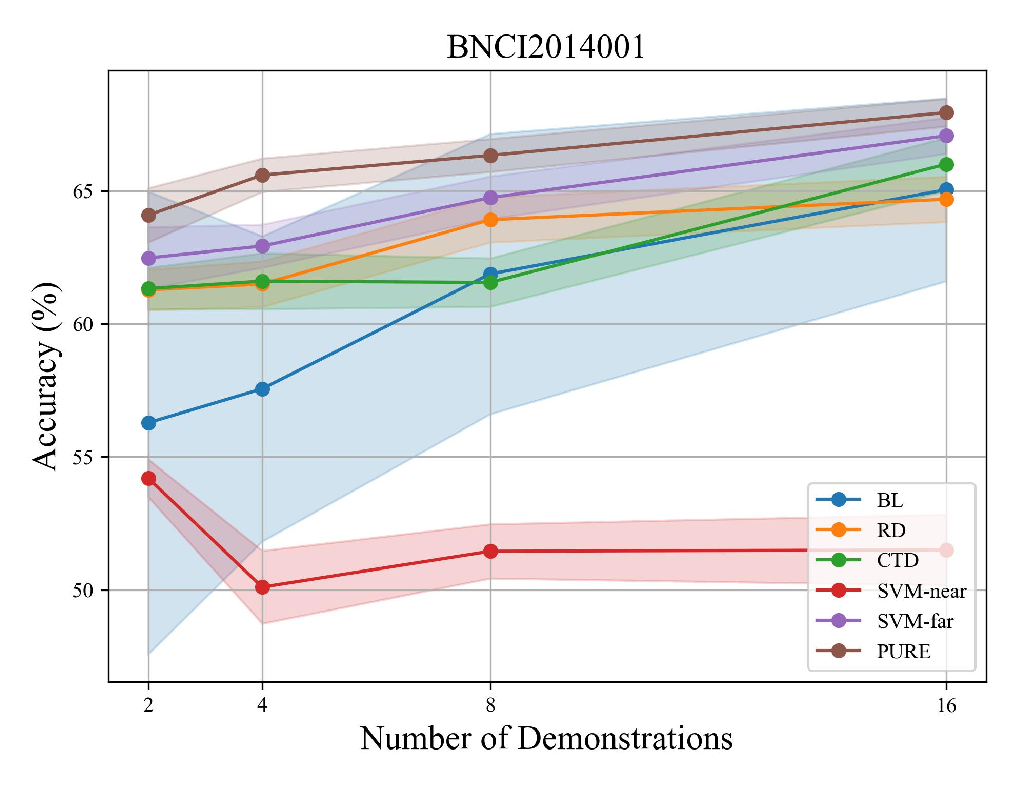
\includegraphics[width=.9\linewidth,clip]{Fig3}
  \caption{Performance under different numbers of in-context demonstrations on BNCI2014001 datasets using BL, RD, CTD, SVM-near, SVM-far, and PGAP approaches. The utilized LLM is Qwen-2.5-14b-instruct-1m.} \label{fig:diff-demo-num}
\end{figure}

\subsection{Comparison of LLMs and CNNs}
To further assess the effectiveness of the proposed LLM-based PGAP, we compared PGAP with existing lightweight CNN models and evaluated its performance on alternative LLMs. We reproduced three traditional CNN models, including EEGNet \cite{Lawhern2018EEGNet}, DeepCNN \cite{deepshallow2017}, and FBCNet \cite{mane2021fbcnet}. For PGAP, DeepSeek-V3 and Qwen-2.5 were utilized for comparative analysis. Experiments were conducted on the BNCI2015001 dataset, and the corresponding results are presented in Table~\ref{tab:deepseek-result}. Observe that:
\begin{enumerate}
\item The proposed LLM-based PGAP consistently outperforms all CNN baselines, highlighting the considerable potential of LLM-based ICL few-shot learning approaches in non-text domains such as EEG signal analysis.
\item The relative performance of DeepSeek-V3 remains consistent with previous performance with Qwen-2.5, confirming the robustness of active selection strategies across different LLM architectures.
\end{enumerate}

\begin{table}[htpb] \centering
\setlength{\tabcolsep}{1mm}
\renewcommand\arraystretch{1}
\caption{Within-subject classification accuracies (\%) on BNCI2015001 using lightweight CNNs and the proposed LLM-based PGAP. The best performance in each subject is marked in bold, and the second best underlined.}
\label{tab:deepseek-result}
\begin{tabular}{c|ccc|cc}
\toprule
\multirow{2.5}{*}{Subject} & \multicolumn{3}{c|}{CNN} & \multicolumn{2}{c}{LLM-based PGAP} \\ \cmidrule(lr){2-6}
 & EEGNet & DeepCNN & FBCNet & Qwen-2.5 & DeepSeek-V3 \\
\midrule
S1 & 93.00  & 78.40  & 86.80 & & \\
S2 & 93.40  & 76.80  & 91.40 & & \\
S3 & 79.80  & 78.00  & 83.00 & & \\
S4 & 80.60  & 63.40  & 80.80 & & \\
S5 & 71.60  & 73.60  & 80.00 & & \\
S6 & 49.20  & 60.40  & 65.80 & & \\
S7 & 73.40  & 62.60  & 66.20 & & \\
S8 & 56.20  & 57.20  & 63.80 & & \\
S9 & 60.20  & 56.20  & 55.00 & & \\
S10 & 56.80  & 57.00  & 55.60 & & \\
S11 & 61.00  & 85.00  & 70.40 & & \\
S12 & 50.40  & 53.60  & 52.00 & & \\
\midrule
Average & 68.80$_{\pm2.14}$ & 66.85$_{\pm2.01}$ & 70.90$_{\pm2.17}$ & & \\
\bottomrule
\end{tabular}
\end{table}

\section{Conclusions}\label{sec:conclusion}
This paper proposed a purity-guided active prompting (PGAP) framework for EEG decoding with LLMs in a few-shot in-context learning scenario. Existing demonstration selection approaches commonly used in NLP and CV domains are often ineffective for EEG data due to its complexity and inherent lack of semantic interpretability. PGAP addresses these limitations by combining domain-specific feature extraction with an active selection strategy based on local same-label purity, selecting compact sets of representative, low-entropy examples. Experiments on multiple EEG datasets across diverse BCI paradigms show that PGAP consistently outperforms random and baseline selection strategies.

\bibliographystyle{IEEEtran}\bibliography{PGAP}

\end{document}
